\chapter{Introduction}

\section{Motivation}

Software bugs are human-made mistakes in a software system that prevent it from working as expected~\cite{ieeestandardglossaryforse}. Existing studies have shown that software bugs cost the global economy billions of dollars every year~\cite{britton2013reversible, zou2018practitioners}. Hundreds of software bugs are submitted to bug-tracking systems like GitHub and JIRA as \textit{bug reports}~\cite{anvik2006should}. These bugs are then triaged, analyzed, and resolved by developers. Developers spend $\sim$50\% of their programming time finding and fixing bugs~\cite{britton2013reversible}. Thus, bug resolution has been one of the major challenges in software maintenance~\cite{zou2018practitioners}.  A recent study suggests that up to 78\% of 32,198 bug reports collected from four open-source projects (e.g., Eclipse, Mozilla, Firefox, GCC) have less than 100 words each, which might not be sufficient (a.k.a., short bug reports)~\cite{zhang2017bug}. These short bug reports required 121 days extra on average for their resolutions as opposed to the well-written bug reports~\cite{zhang2017bug}. That is, missing information in bug reports could lead to their delayed resolution~\cite{zhang2017bug}. According to a recent survey~\cite{zou2018practitioners}, 77\%  of 327 software practitioners (e.g., developers, testers, managers) from the major technology companies (e.g., Google, Meta, Amazon, Microsoft) consider missing information as a major problem and emphasize on complementing bug reports with useful information (e.g., steps to reproduce, environmental configuration)~\cite{zou2018practitioners}. Missing information has also been found to be a key factor behind the non-reproducibility of software bugs~\cite{rahman2020some}. Thus, missing information has been a major challenge and complementing the bug reports with relevant information would greatly benefit the developers in their bug resolution.\par
\begin{figure} [!htbp]
    \centering 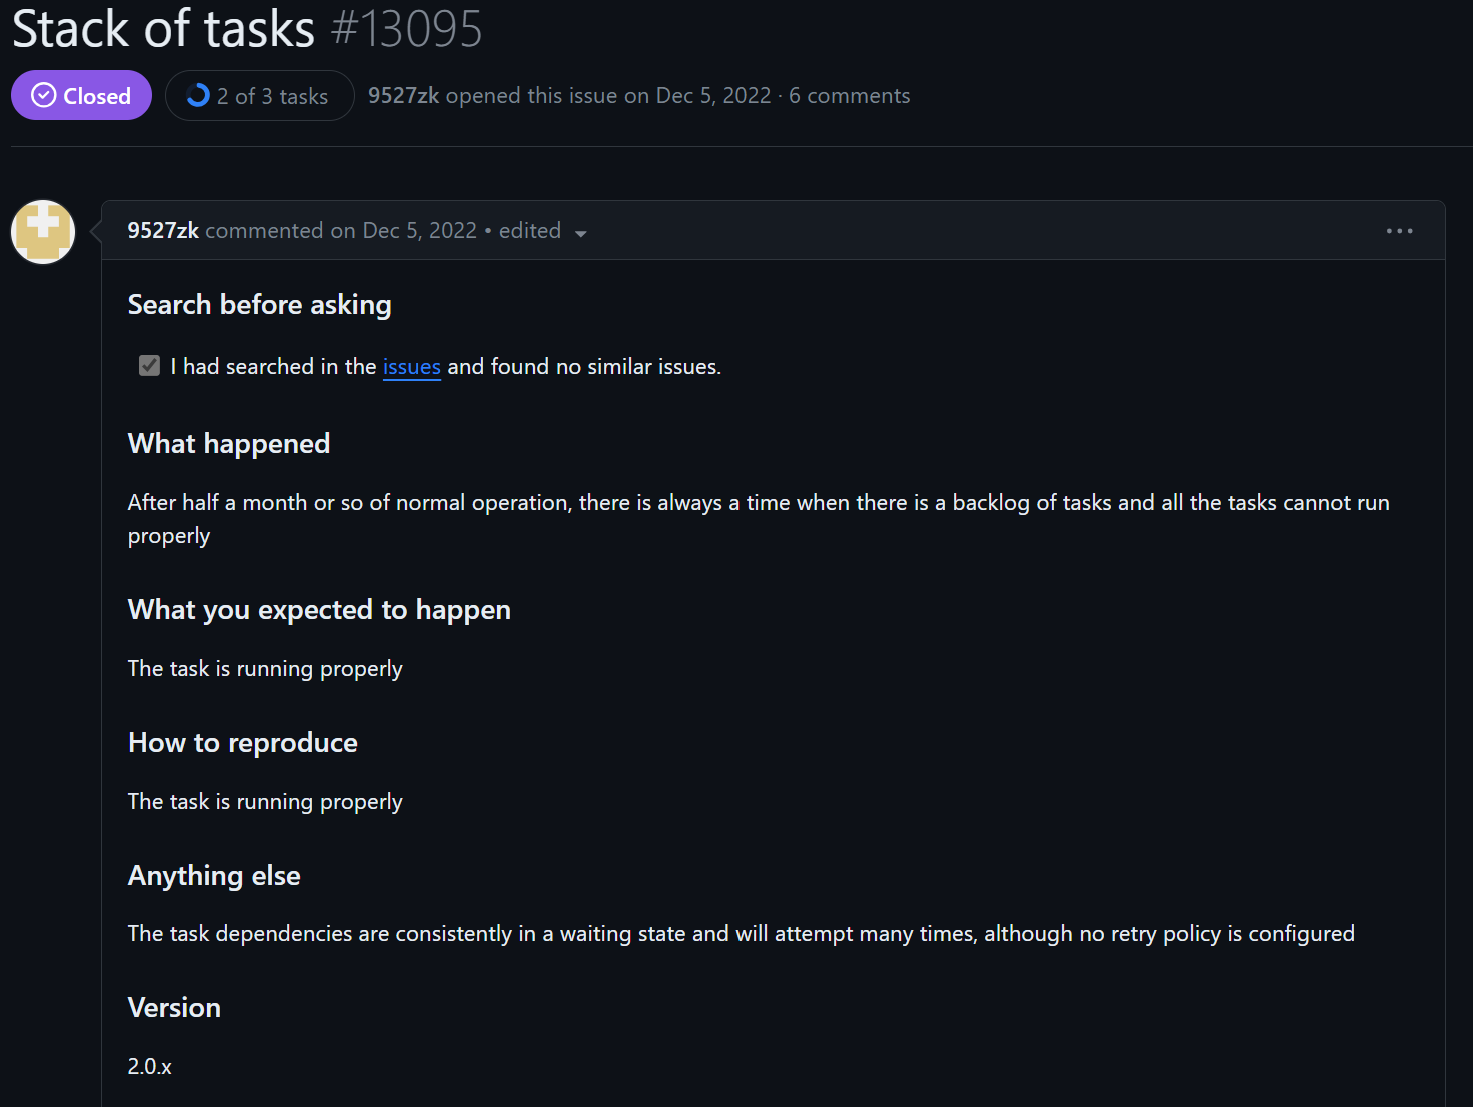
\includegraphics[width=0.8\textwidth]{images/intro_missing_info_eg.png} 
    \caption{An example bug report with missing information (ID \#13095)}
    \label{fig:missinginfo}
\end{figure}

Ideally, bug reports should contain all the information, such as system configuration, expected behaviour, observed behaviour, and reproducing steps that help a developer resolve a bug~\cite{chaparro2017detecting}. However, in practice, they often do not contain all the required information for reproducing or resolving a bug~\cite{chaparro2017detecting}. Let us consider the example bug report in Fig. \ref{fig:missinginfo}. It discusses a task backlog problem where the task dependencies are consistently in a waiting state. However the reporter does not provide any system configuration details, logs or steps to reproduce. As a result, the report was later marked as ``needs more information" and then closed. According to existing literature~\cite{chaparro2017detecting},  64.8\% of bug reports do not contain any expected behaviour of target software systems, and 48.6\% of them do not explicitly describe the steps to reproduce a bug. Many software projects on GitHub now require the bug reports to adhere to specific templates or standard guidelines~\cite{githubguidelines}. However, many bug reporters might fail to comply with them and might not be able to provide all the information during report submission~\cite {imran2021automatically}. Developers thus often pose \textit{follow-up} questions to bug reporters soliciting the missing information. Unfortunately, the bug reporters often find it challenging to answer the follow-up questions in a timely fashion, according to a recent developer survey ~\cite{rahman2020some}. Such a lack of responses could lead to non-reproducible or unresolved bugs~\cite{breu2010information}. However, there has been only a little research investigating the follow-up questions from bug reports or their answers.

\begin{figure}[!htpb]
  \centering
  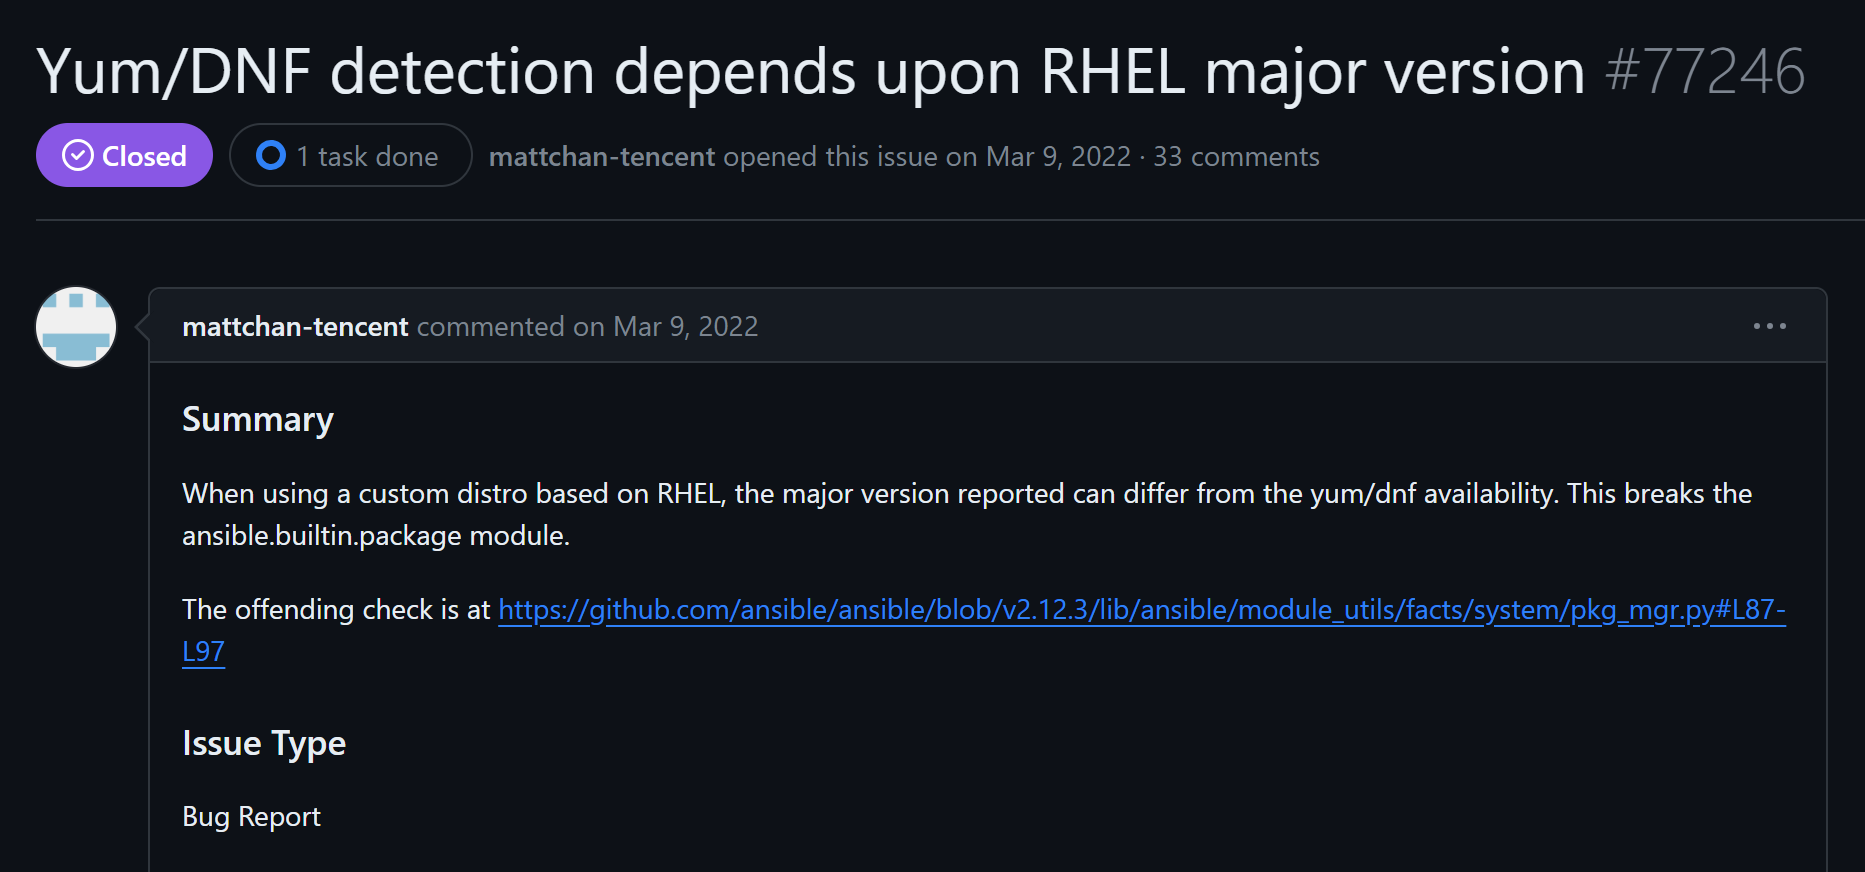
\includegraphics[width=0.8\textwidth]{images/not_readable_bug_report.png}
  \caption{ An example bug report (ID \#77246)}
  \label{Intro-fig:notreadbleBR}
\end{figure}

Answers to the follow-up questions provide more contextual information regarding a reported bug, which could help the developers resolve the bug. However, newcomers or novice developers to a project might need additional help to accurately understand or resolve a bug. In particular, complex contextual information and the incomplete or inaccurate content in bug reports could make bug understanding a challenging task~\cite{velly2013towards}. Let us consider the example bug report in Fig. \ref{Intro-fig:notreadbleBR}. The bug report uses several software-specific terms such as ``custom distro'', ``RHEL'' and ``yum/dnf". It discusses the ansible version mismatch between the custom distribution of Red Hat Enterprise Linux (RHEL) and the Yellowdog Updater Modified (yum)/dandified YUM (dnf) package management tool. To a newcomer, all these terminologies could be daunting and discouraging. However, decoding them is essential to understand and diagnose the reported bug. 
% This discrepancy poses a challenge, potentially causing a malfunction in the ansible.builtin.package module, which relies on accurate version information for proper execution. 
According to an existing study~\cite{guizani2021long}, even with prior experience, developers often struggle to acquire a comprehensive understanding of any application domain and understand the discussions from a bug report. Thus, a lack of explanation for the domain-specific terms or jargon could be a major issue towards bug understandability.

\section{Problem Statement}

Bug reports are a valuable resource for software maintenance and continuous evolution. Over the last few decades, there has been extensive research to support various bug report management tasks, including bug triage ~\cite{zhao2019unified}, ~\cite{bodden2017proceedings}, issue report classification ~\cite{thung2012automatic}, ~\cite{nayrolles2018towards}, duplicate bug report detection~\cite{nguyen2012duplicate, chaparro2019reformulating}, and bug localization ~\cite{zhang2019finelocator}, ~\cite{xiao2019improving}. However, the problem of missing information or domain-specific jargon in bug reports has not been comprehensively studied or addressed. Given the evidence above, adding complementary information to deficient bug reports could greatly benefit software practitioners in their work.\par

There have been existing studies that provide complementary information through Question Answering (QA) to support various software engineering tasks. Tian et al.~\cite{tian2017apibot} designed APIBot that can answer questions related to an API by analyzing relevant API documentation. Bansal et al.~\cite{bansal2021neural} designed a context-aware QA system to answer basic questions about subroutines. Lu et al.~\cite{lu2021beat} proposed a QA approach that can provide answers by executing structured queries generated from bug templates. However, there has been only a little research investigating the follow-up questions from bug reports or their answers. Breu et al.~\cite{breu2010information} first conducted a mix of quantitative and qualitative analysis on follow-up questions and found that 32.34\% of the questions were never responded to. They suggest that the questions in the bug reports were critical to the effective triaging, reproduction and resolution of a bug. Recently, Imran et al.~\cite{imran2021automatically} proposed a technique that recommends follow-up questions against a deficient bug report using structured information retrieval. Although both studies above deal with the follow-up questions from a bug report and are a source of inspiration, they do not answer the questions.\par

There have been existing studies to support newcomers or inexperienced developers who may struggle to comprehend software bug reports. An existing survey by Tan et al.~\cite{tan2020first} suggests that a clear description of a bug that does not rely on in-depth domain knowledge is necessary to help newcomers understand and resolve the bug. Recently, Correa et al.~\cite{correa2013samekana} suggest that the inclusion of web links (to external knowledge sources or artifacts) in the issue tracker discussion can benefit the developers. Zhang et al.~\cite{zhang2017bug} propose to supplement a bug report with a list of sorted sentences that are extracted from past, relevant bug reports. Dit et al.~\cite{dit2008improving} proposed a technique that recommends relevant comments so that the developers can make explicit connections between the recommended comments and existing ones. Such connections could help the developers better understand a bug report. While the above approaches offer complementary information to support bug understanding, they do not focus on the domain-specific terms or jargon, which warrants for further investigation.\par

% research problem without lit
Given the above discussions, missing information is one of the key factors that affect developers when comprehending software bug reports and could lead to delayed bug delayed reproduction and resolution. It affects bug reports in two different ways. First, bug reports often do not contain sufficient information for timely resolution. Developers thus pose follow-up questions asking the bug reporter for missing information. However, bug reporters or any user facing a similar bug may find it challenging to answer them due to a lack of domain-knowledge. Second, bug reports may contain domain-specific terms or jargon that may not be well understood by novice or newcomer developers. Traditional bug tracking systems do not provide any support to comprehend such domain-specific terms or jargon. To the best of our knowledge, existing literature might also not be sufficient to enhance the bug reports plagued by missing information. We thus perform two studies to complement such deficient bug reports with missing information using automated tools and technologies. \par

 
\section{Our Contribution}
In this thesis, we propose and evaluate two novel techniques that support developers in bug resolution by complementing a deficient bug report in two different ways.

In our first study, we propose a novel technique --- \textit{BugMentor} --- that can offer relevant answers to follow-up questions from bug reports by combining structured information retrieval and neural text generation. First, we capture textually relevant questions, answers, and bug reports against a follow-up question using structured information retrieval~\cite{saha2013improving}. Then we capture each item's embeddings using Word2Vec~\cite{efstathiou2018word} and re-rank them based on their semantic relevance to the question. Second, we generate meaningful answers to the follow-up question by leveraging the ranked items above as \textit{context} with a neural text-generation technique (e.g., CodeT5).

We evaluate answers from \textit{BugMentor} using four performance metrics ---  BLEU score~\cite{papineni2002bleu}, METEOR~\cite{banerjee2005meteor}, Semantic Similarity~\cite{haque2022semantic}, and WMD~\cite{huang2016supervised}. We achieve a BLEU score of 34.12 which indicates that our generated answers are \textit{understandable} to \textit{good} according to Google AutoML documentation~\cite{automldoc}. We also conduct an ablation study to justify our combination of structured information retrieval and neural text generation in BugMentor. We find that BugMentor can capture a rich context leveraging structured information retrieval and thus can generate meaningful answers. BugMentor also outperforms all three baselines --- Lucene~\cite{mccandless2010lucene}, CodeT5~\cite{wang2021codet5}, AnswerBot~\cite{xu2017answerbot} --- in all four metrics.  To further demonstrate its benefit, we conduct a developer study involving 10 participants. According to the participants, the answers from BugMentor were more accurate, more precise, more concise and more useful compared to the baseline answers.


In our second study, we propose -- \textit{BugEnricher} -- a novel technique that can enhance bug reports with meaningful explanations to their domain-specific terms or jargon using neural text generation. First, we collect thousands of domain-specific vocabulary and their explanations from three different sources -- StackOverflow, API documentation, and glossary. Second, we fine tune the T5 model~\cite{raffel2020exploring} on our collected vocabulary and explanations. Third, we use \acrshort{TF-IDF} to extract the infrequent domain-specific terms from each bug report. Finally, we generate natural language explanations to the domain-specific terms or jargon using our fine-tuned T5 model. \par

Our evaluation using three performance metrics shows that \textit{BugEnricher} can generate \textit{understandable} and \textit{good} explanations according to Google’s standard, and can outperform two existing baselines --- T5~\cite{raffel2020exploring} and AnswerBot~\cite{xu2017answerbot} --- from the literature. To further demonstrate the benefit of our explanations, we conduct a case study using the bug reports enriched with explanations. We evaluate the performances of an existing technique~\cite{yang2012duplication} for duplicate bug report detection that is impacted by the problem of textually dissimilarity~\cite{jahan2023towards}. We find that the enriched bug reports were able to improve the performances of the existing technique in detecting textually dissimilar duplicate bug reports.\par

Given the empirical evidence, our proposed techniques have the potential to significantly improve the bug report management and their resolution.

\section{Related Publications}
Several parts of this thesis are either submitted or ready to be submitted to different conferences.
We provide a list of papers here. In each of these papers, I am the primary author, and all the studies were conducted by me under the supervision of Dr. Masud Rahman. While I wrote these papers, the co-author took part in advising, editing, and reviewing the papers.
\begin{itemize}
    \item \emph{Usmi Mukherjee} and M. Masudur Rahman. \emph{Answering Follow-up Questions from Bug Reports Leveraging Structured Information Retrieval with Neural Text Generation}. In Proceedings of the 47th International Conference on Software Engineering (ICSE 2025), pp.13, Ottawa, Canada, April-May 2025.(Pre-submission)
\end{itemize}

\begin{itemize}
    \item \emph{Usmi Mukherjee} and M. Masudur Rahman. \emph{BugEnricher: Explaining Domain-specific Terms and Jargon from Bug Reports with Neural Machine Translation}. In Proceeding of the 40th IEEE International Conference on Software Maintenance and Evolution (ICSME 2024), pp. 12, Flagstaff, Arizona, October 2024 (Pre-submission).
\end{itemize}

\section{Outline of the Thesis}

The thesis contains five chapters in total.
To complement missing information in bug report effectively, we conduct two independent but interrelated studies, and this section outlines different chapters of the thesis.

\begin{itemize}
    \item Chapter 2 discusses several background concepts (e.g., embedding, transformers, neural language modeling) that are required to follow the rest of the thesis.

    \item Chapter 3 discusses our first study that proposes \textit{BugMentor}, a novel approach that combines neural text generation (e.g., CodeT5) and structured information retrieval to generate appropriate answers to the follow-up questions.

    \sloppy
    \item Chapter 4 discusses our second study that proposes \emph{BugEnricher}, a novel transformer-based generative model that generates natural language explanations for software-specific terms in Bug Reports.

    \item Chapter 5 concludes the thesis with a list of directions for future works.
\end{itemize}